\section{Produktprincip}
    \subsection{Målgruppe}
    Efter som det nuværende Lectio bliver anvendt af en stor del af landets gymnasier, er vores målgruppe derved alle landets gymnasier--nemlig også potentielle kunder (gymnasier) der
    muligvis ville være interesseret i at anvende vores Lectio applikation. 
    

    \subsection{Kravspecifikation}
    Kravene for vores applikation er følgende: 
    
    \begin{itemize}
        \item Applikationen skal have alle de samme core-features som det originale Lectio
        \item Applikationen skal være let overskuelig og nemt orienterbart for brugerne
        \begin{itemize}
            \item Applikationen skal således være simplere end sin forløber
        \end{itemize}
        \item Applikationen skal indeholde et Lokale-Booking-System/Fraværsregistreringssystem/Dørsystem 
        \begin{itemize}
            \item Applikationen skal have forbedret fraværsregistrering
            \item Applikationen skal give alle eleverne et digitalt persona i sammenspil med fraværsregistreringssystemet. 
            \item Et komplet dørsystem som låses/låses op med RFID kort (på sigt ens mobiltelefon). 
        \end{itemize}
    \end{itemize}

    \subsection{Kort om konkurrenter}
        Lectio har ingen umiddelbare konkurrenter, vi kender, udover Aula, men det henvender sig til folkeskoler og har ikke envidere fildelingsinfrastruktur. Vi tror også, at problemet med Lectio stammer fra det faktum, at Lectio har et de-facto monopol på IT-løsninger målrettet gymnasier.

    \subsection{Løsningsforslag}
        \subsubsection{Lectio rework}
        For at løse problemet med det forældede Lectio har vi besluttet at lave et komplet rework (dvs. genopbyggelse af softwaren, men med samme kernefunktionalitet) af Lectio applikationen.

        Vi har udarbejdet skitser for at kvalificerer vores produktudformning. Sktitserne viser de vigtigste sider af vores Lectio rework.
        \begin{figure}[H]
            \centering
            \resizebox{!}{12cm}{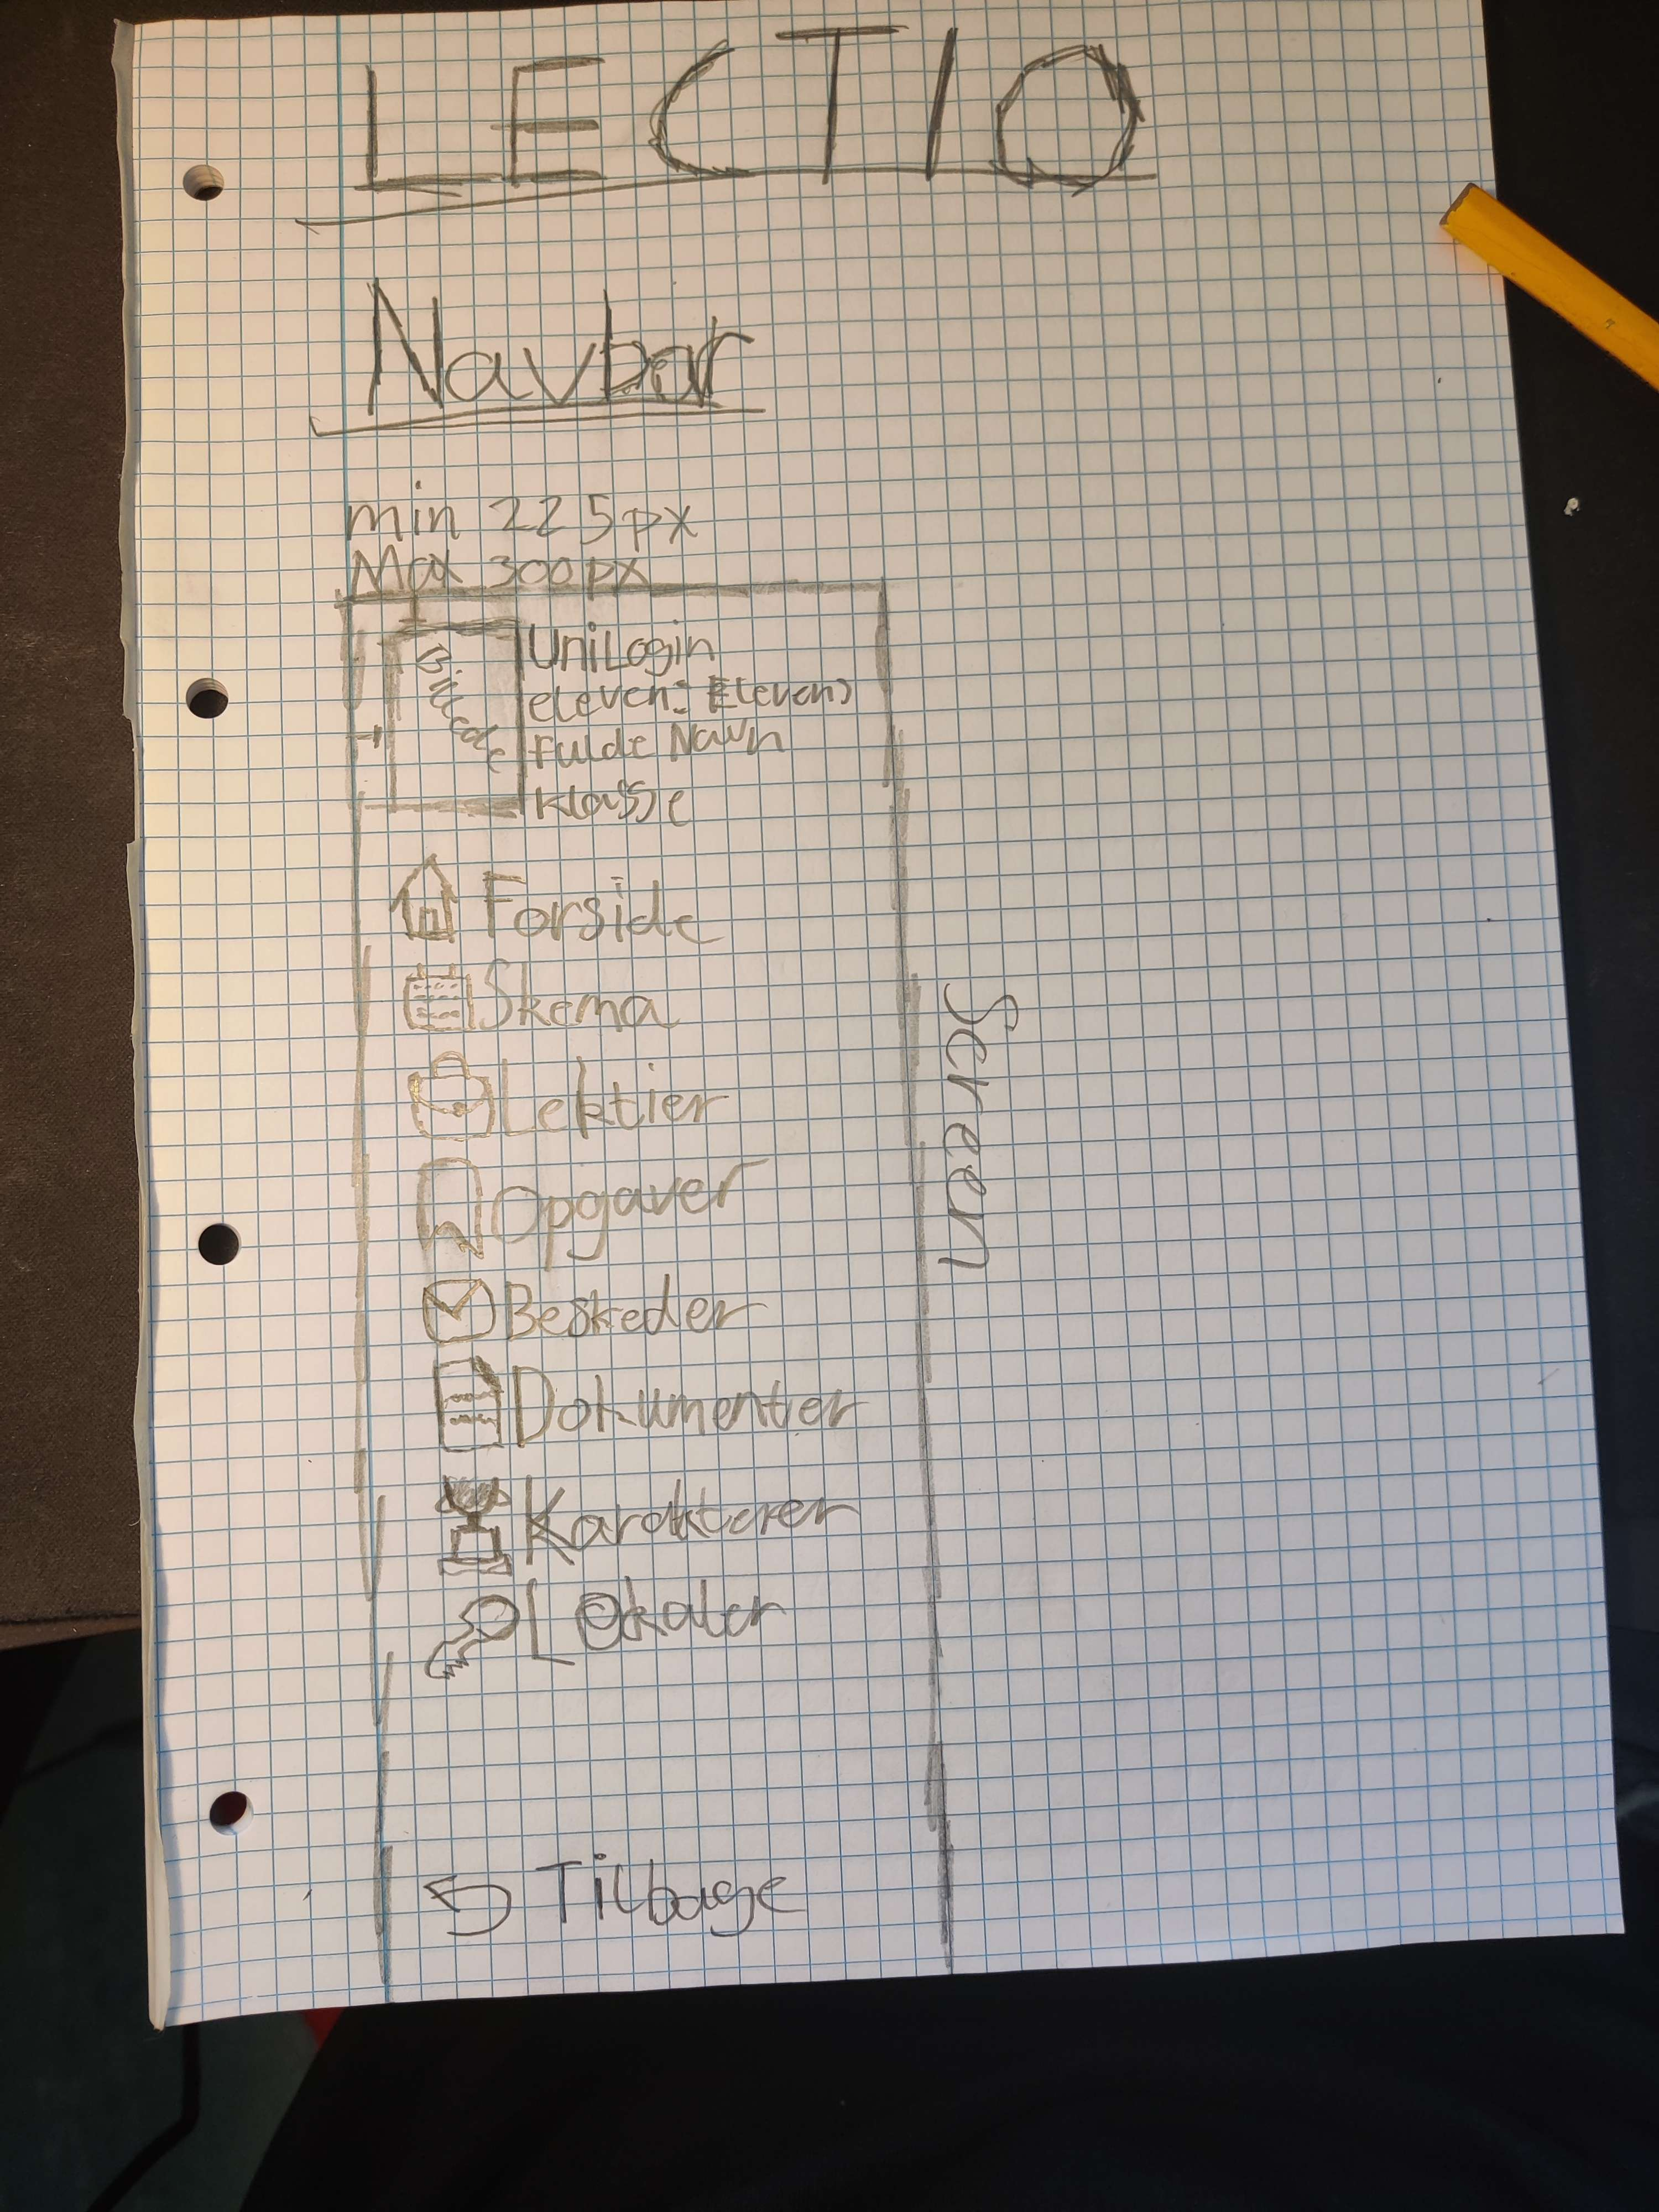
\includegraphics[]{assets/lectio_navbar_skitse.jpg}}
            \caption{Viser Lectioreworkets navigationsbarkomponent - bjælken, brugeren intergerer med}
        \end{figure}

        \begin{figure}[H]
            \centering
            \resizebox{!}{10cm}{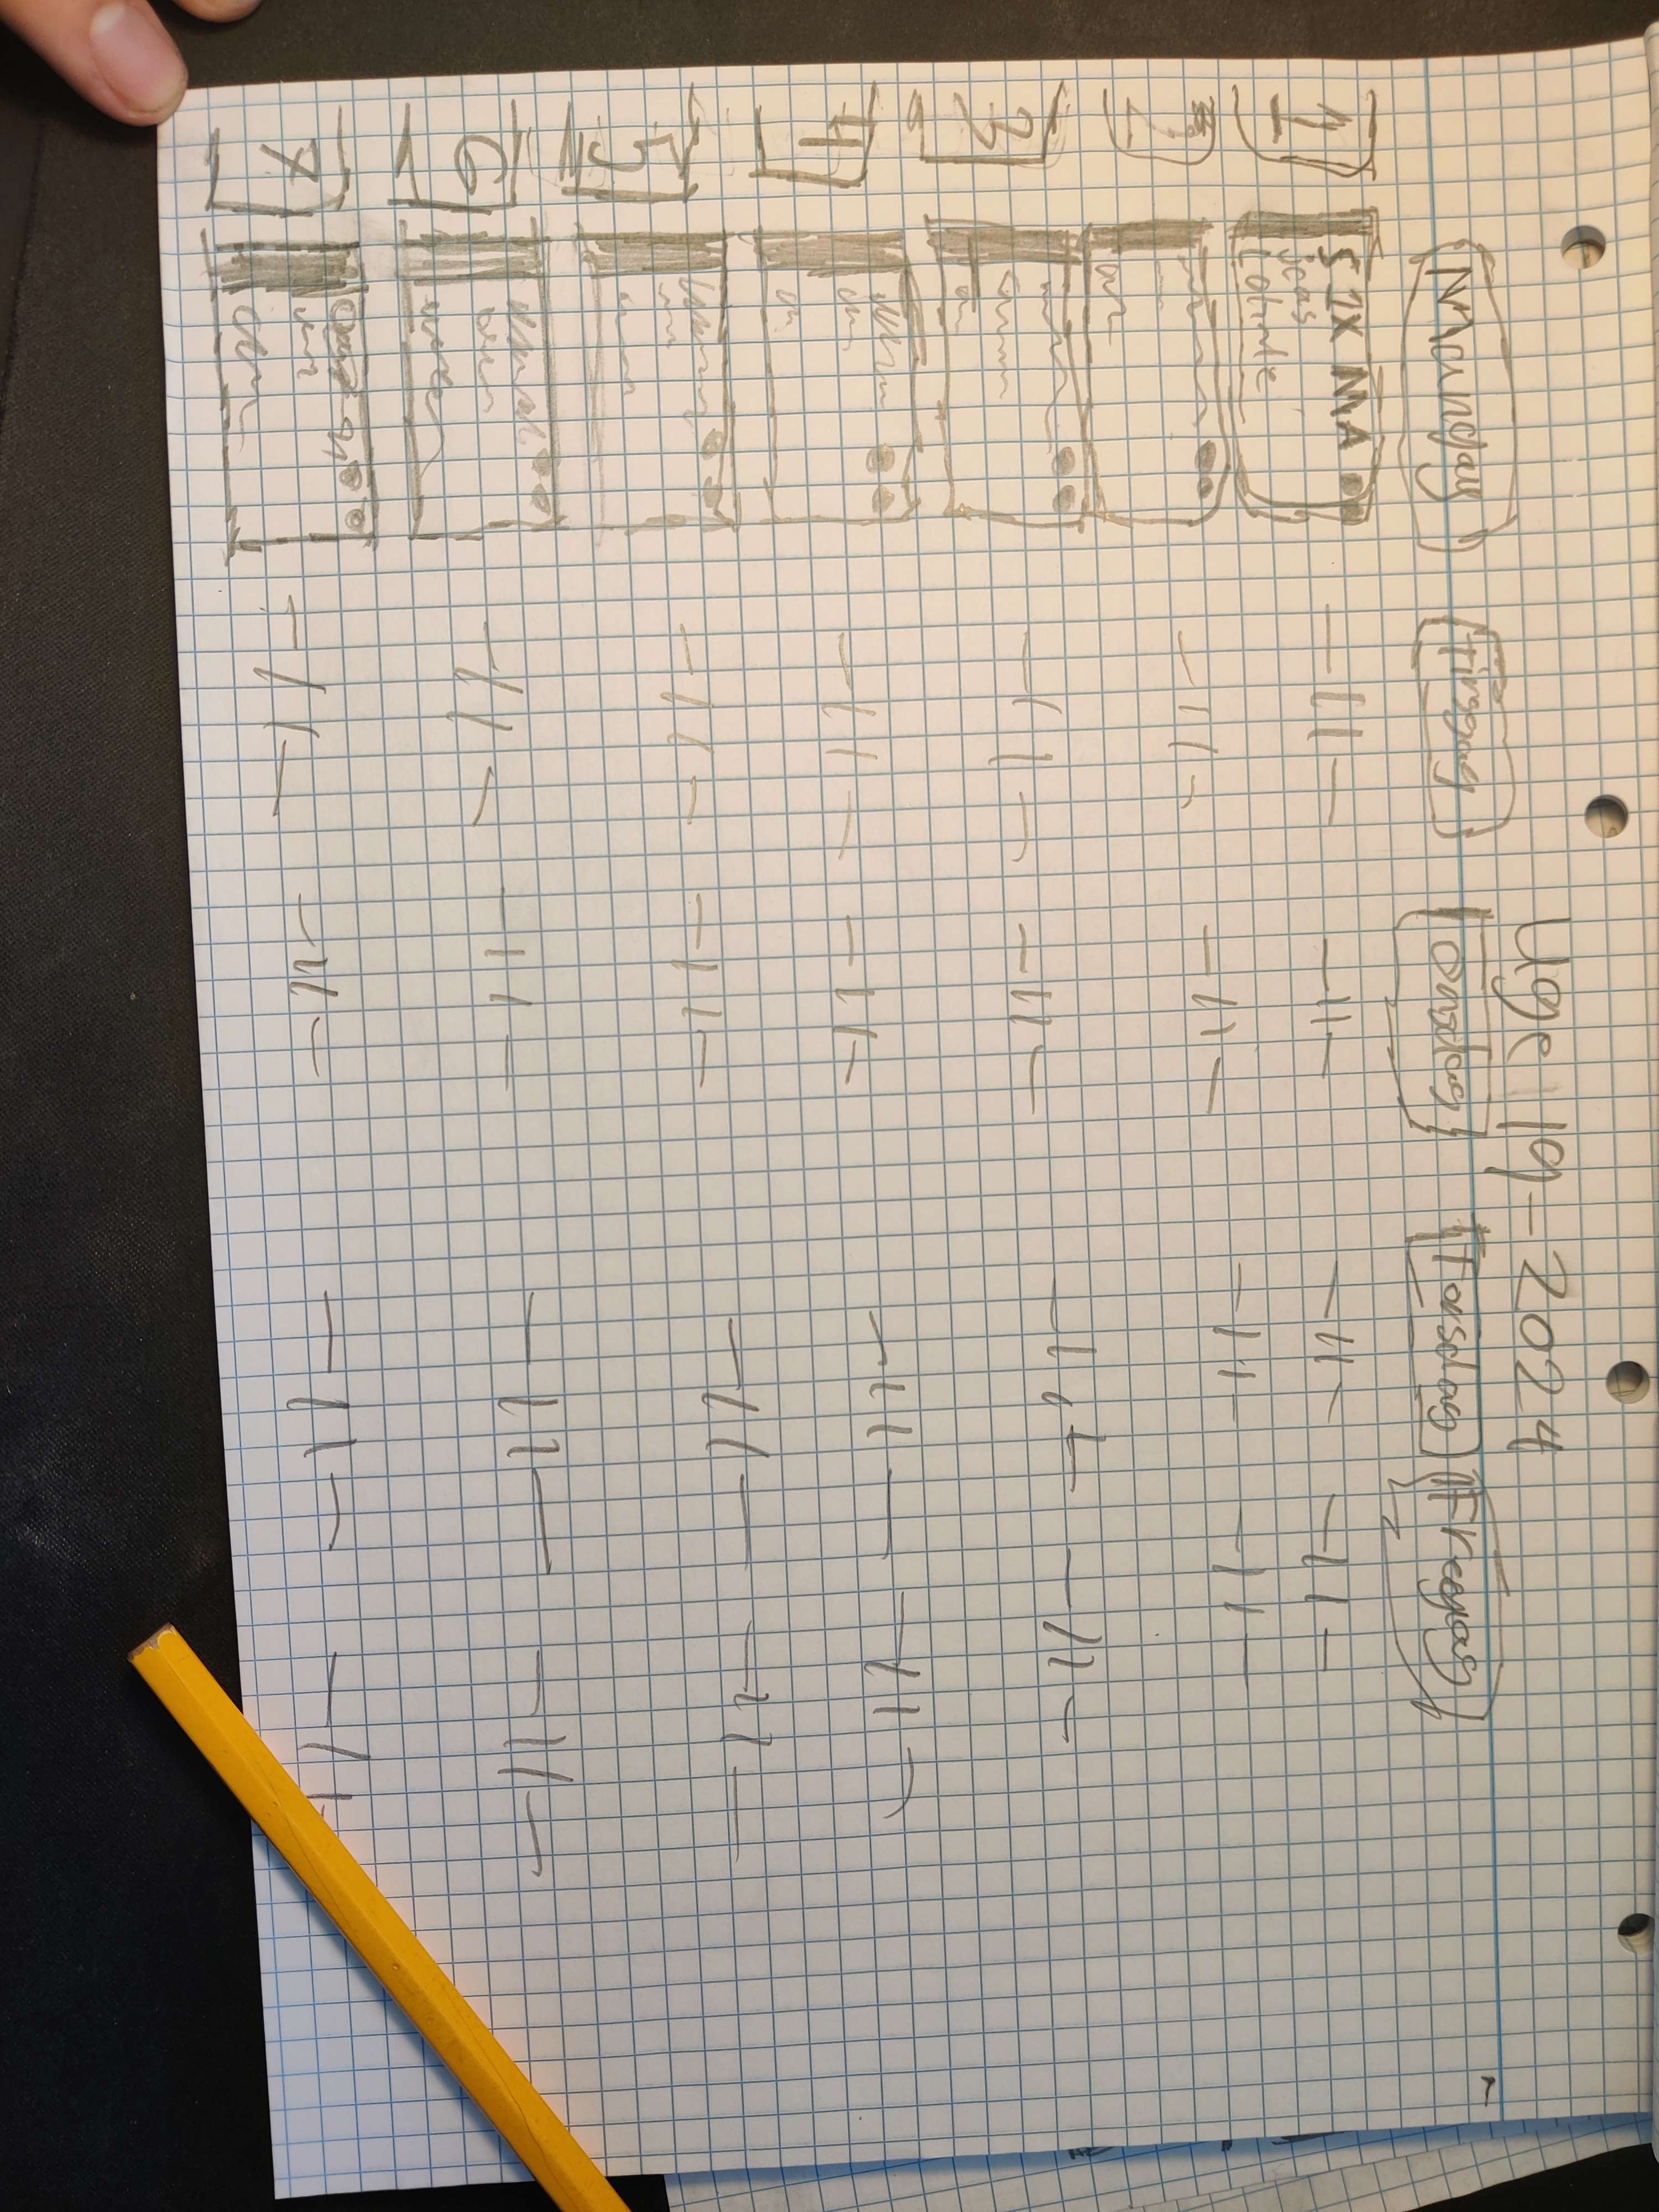
\includegraphics[angle =90]{assets/lectio_skema_skite.jpg}}
            \caption{Viser Lectioreworkets skema side}
        \end{figure}

        De resterende skitser, vi har udarbejdet, fremgår af appendikssektionen \ref{appendix:arbejdsskitser}.

        \subsubsection{RFID-Løsning}
        For at tage hånd om problemet med spildtid i form af fraværstagning, fejlagtig fraværstagning m.v. har vi valgt at lave et dør/fraværssystem, som når man om morgnen møder ind, scanner man sig ind med sit ID-kort eller sit
        digitale ID-kort med sin mobiltelefon på fraværsregistreringssystemet som er i klassen.  
        Lokale-Booking-Systemet fungerer (i ideen--se evalueringen \ref{sec:konklusion}) i sammenspil med den nye Lectio applikation, så kan igennem applikationen booke et lokale også med sit ID-kort
        låse lokalet op i det tidsrum man har booket det pågældene lokale. Web løsningen ses skitseret forneden:

        \begin{figure}[H]
            \centering
            \resizebox{!}{10cm}{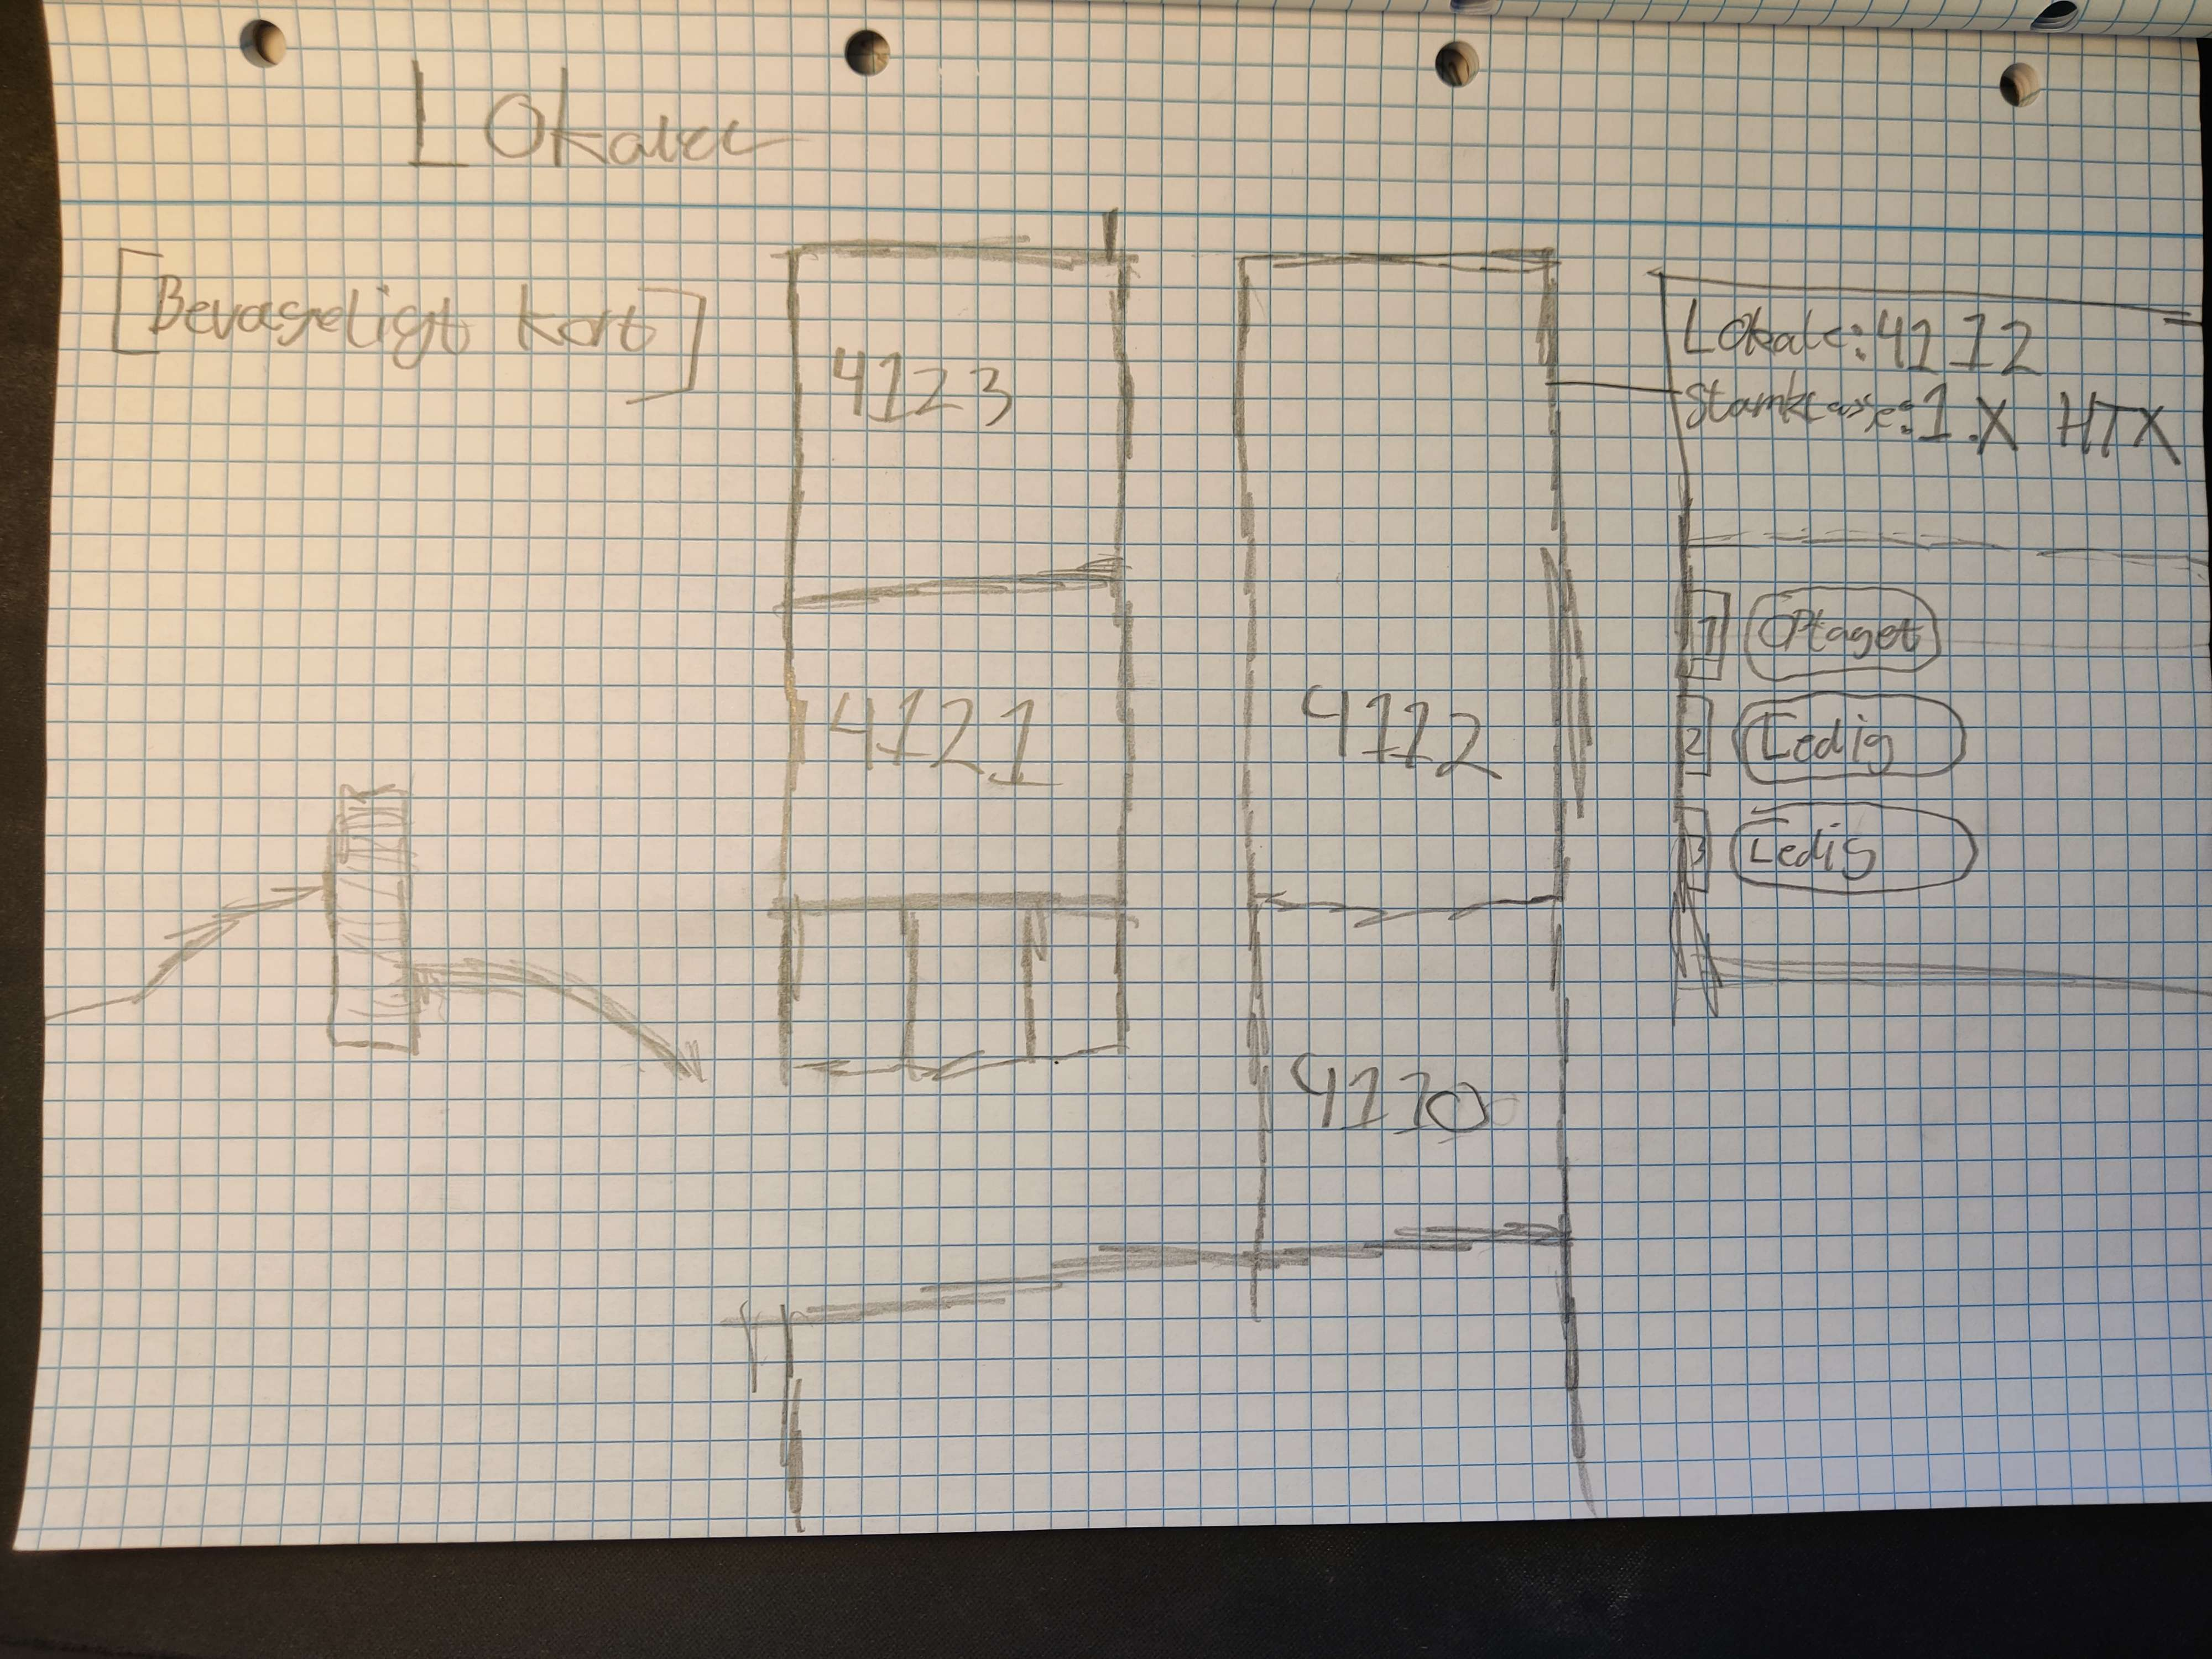
\includegraphics{assets/lectio_lokaler_skitse.jpg}}
            \caption{Viser Skitse af Booking siden på samme webapplikation som Lectio Reworket}
        \end{figure}
